\section{Task: Associate Target Reports}
\label{sec:task_associate_tr} 

This task allows creation of UTNs (Unique Target Numbers) and target report association based on Mode S Addresses, Mode A/C codes and position information. \\

Each target found is identified by a UTN, and groups together all reference/tracker/sensor target reports (which can) be associated to this target.

Please note that if usage of UTNs is not needed, these step does not have to be performed. If usage of the evaluation feature is wanted, running this task is required. \\

\begin{figure}[H]
  \hspace*{-2.5cm}
    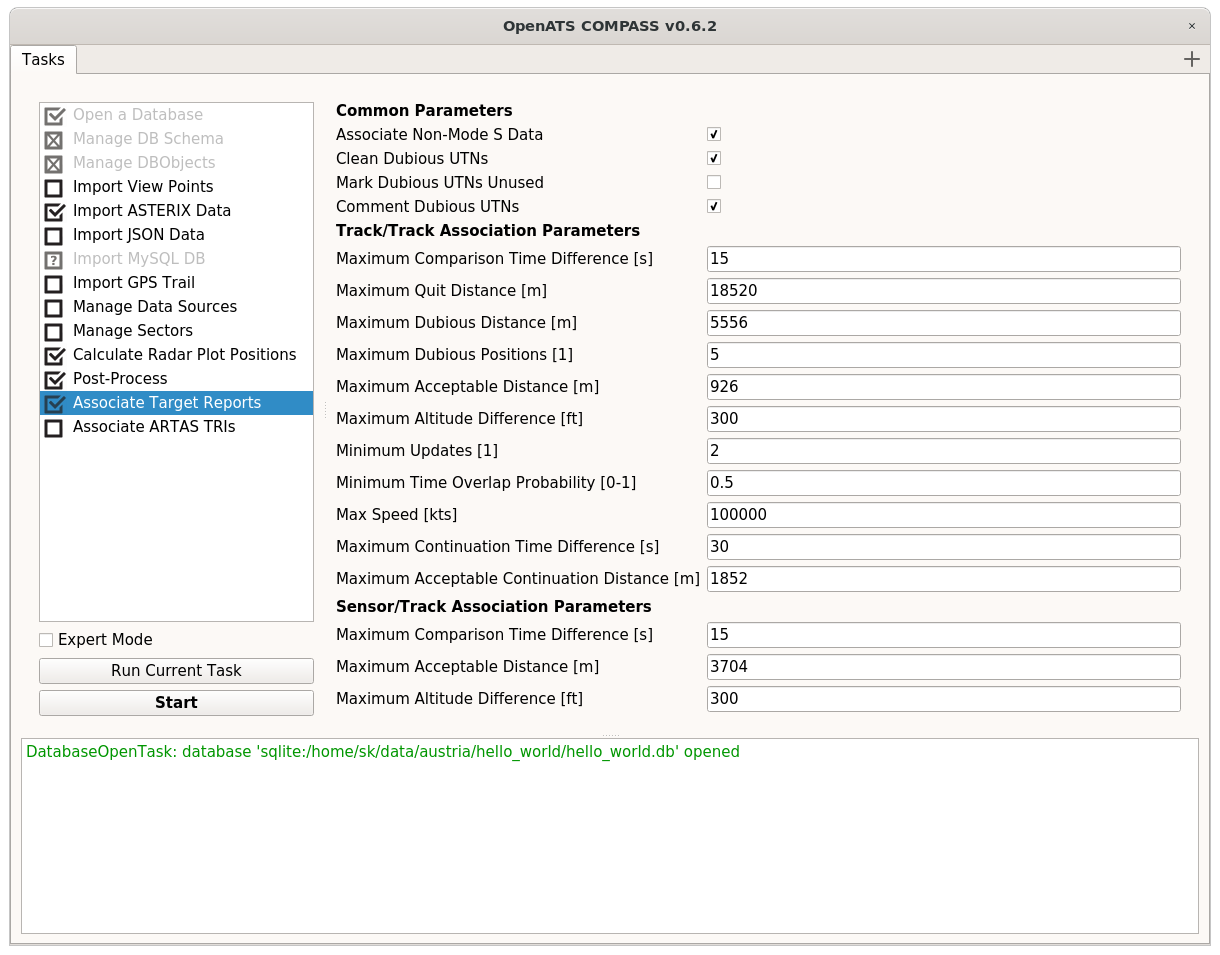
\includegraphics[width=19cm]{../screenshots/tr_association_config.png}
  \caption{Task: Associate Target Reports}
\end{figure}

The configuration of the task requires knowledge of the internals of how the associations are made. As a brief description, the following steps are performed:

\begin{itemize}
\item Delete all previously existing associations
\item Load all target reports, per data source
\item Add UTNs based on reference (RefTraj) data sources
\item Add UTNs based on Tracker data sources
\item Add UTNs based on remaining sensor data sources
\end{itemize}
\ \\

Common parameters
\begin{table}[H]
  \center
  \begin{tabular}{ | l | l | l |}
    \hline
    \textbf{Parameter} & \textbf{Default Value} &  \textbf{Description} \\ \hline
    Associate Non-Mode S Data & true & - \\ \hline
    Clean Dubious UTNs & true & - \\ \hline
    Mark Dubious UTNs Unused & false & - \\ \hline
    Comment Dubious UTNs & true & - \\ \hline
  \end{tabular}
  \caption{Map widget view operations in Navigate mode}
\end{table}

    Track/Track Association Parameters
    Maximum Comparison Time Difference [s] 15.0
    Maximum Quit Distance [m]
    Maximum Dubious Distance [m]
    Maximum Dubious Positions [1]
    Maximum Acceptable Distance [m]
    Maximum Altitude Difference [ft]
    Minimum Updates [1]
    Minimum Time Overlap Probability [0-1]
    Max Speed [kts]
    Maximum Continuation Time Difference [s]
    Maximum Acceptable Continuation Distance [m]

    Sensor/Track Association Parameters
    Maximum Comparison Time Difference [s]
    Maximum Acceptable Distance [m]
    Maximum Altitude Difference [ft]


\subsection{Reference/Tracker UTN Creation}

\subsection{Sensor UTN Creation}

The UTNs are created by simply associating all target reports (from all DBObjects) by their Mode S address. Each found unique Mode S target address is assigned a unique UTN, to which in turn all target reports with this address are associated. \\

Target reports without a Mode S address are not associated to any UTN. \\

The author is aware that this does not allow a lot of meaningful use cases, so this task will be improved in the near future to include association based on local track numbers, Mode A/C codes and position metrics. \\

To run the task, click the 'Run Current Task' button. After the assocations are saved, the task is done:

\begin{figure}[H]
  \center
    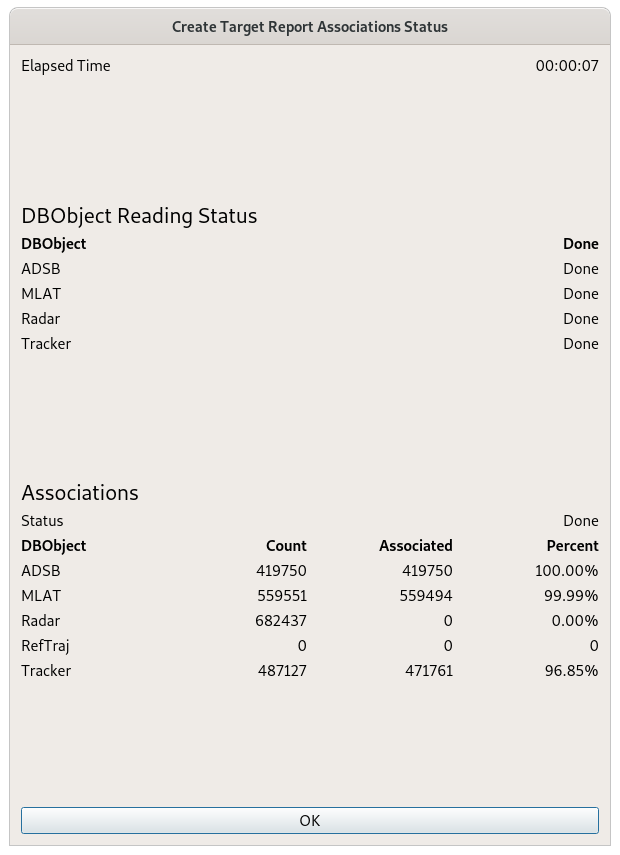
\includegraphics[width=11cm]{../screenshots/tr_association_done.png}
\end{figure}
